\begin{figure}[!h]
\chapter{Class Diagrams and Interface Specifications}
\section{Financial Adaptor Class Diagram}
\centering
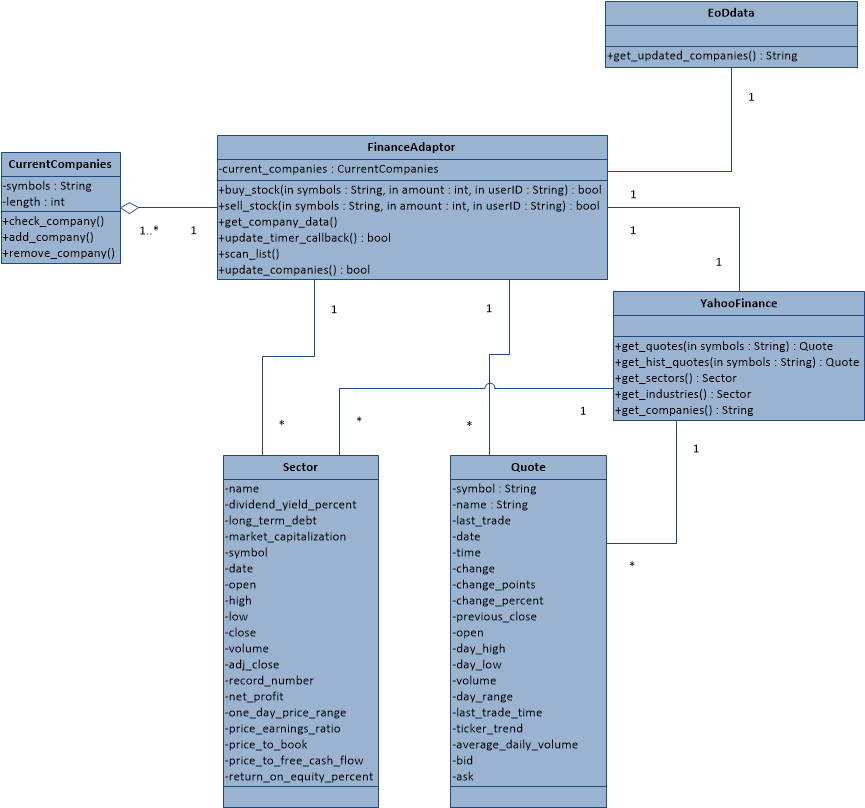
\includegraphics[width=5.5in]{./Diagrams/DomainModel/Financialdomainmodel.png}
\end{figure}

\clearpage

\section{Financial Adaptor Data Types and Operation Signatures}
\subsection{Finance Adaptor}
{\bfseries Attributes} \\*
Our Finance Adaptor performs the functions of validating user queries with 
existing stock symbols, companies, and/or sectors, then mediating between
the Capital Games web server and Yahoo! Finance, enabling our fantasy league
to be playable in real time.  To accomplish data validation, a portion of the
Capital Games database is updated regularly to keep our fantasy stock market
league up to date based off of EODData, an API allowing for the reference to
an up-to-date list of all stock-symbols, company names, and sector/industries. \\* \\*
{\bfseries --- current\_companies : CurrentCompanies } \\*
	This is a reference to a database table updated via an external website, EoDdata,
	that verifies user queries with actual stock symbols, and/or 
	company/sector/inddustry names depending on the user query. \\*\\*

{\bfseries Methods} \\*
Most methods are boolean, returning either success or failure regardng data retrieval.
All other methods are voids, with no arguments, used for executing a specific function. \\* \\*
{\bfseries + buy\_stock (in symbols : String, in amount : int, in userID : String) : bool } \\*
	Method called to buy stock; a typical method that would require the user to query
	up-to-date stock market information via our adaptor. \\*
{\bfseries + sell\_stock (in symbols : String, in amount : int, in userID : String) : bool } \\*
	Method called to sell stock; a typical method that would require the user to query
	up-to-date stock market information via our adaptor. \\*
{\bfseries + get\_company\_data() } \\* 
	This method returns all information available on Yahoo! Finance regarding a user's queried 
	stock. \\*
{\bfseries + update\_timer\_callback() : bool } \\*
	An internal timer signaling the stock query from Yahoo! Finance.  \\*
{\bfseries + scan_list()  }\\*
	This method checks against the Capital Games' database. \\*
{\bfseries + update\_companies() : bool } \\*

	This method updates the information in the Caital Games' database from both Yahoo! Finance
	and EODData. \\*
\subsection{Current Companies}
 

{\bfseries Attributes} \\*
Current Companies is the database table that our Finance Adaptor actually checks against 
when validating user queries. At a regular interval (based on method update_timer_callback from
the Finance Adaptor, the Finance Adaptor retrieves data from EODData to update the Current 
Companies database table.) This is done to maximize efficiency by minimizing the amount of time
the adaptor must retrieve data from EODData. \\* \\*
{\bfseries --- symbols : String \\* }
	This is all stock symbols. \\* 
{\bfseries --- length : integer \\* }
	This defines how many total stock symbols are on the list. \\* 


{\bfseries Methods} \\*
All of these methods are invoked after the stock symbol or company name has been validated.
All methods perform queries regarding updating the Current Companies tabe. \\* \\* 
{\bfseries + check\_company () } \\*
	This method returns all informaton regarding a stock, to be parsed by the Finance Adaptor to
	retrieve what the user is querying for. \\*
{\bfseries + add\_company () } \\*
	Method called to add a company to the database in cases such as Initial Public Offering of
	shares. \\*
{\bfseries + remove\_company() } \\*
	Method called to remove a company from the database in case of acquisition. \\*

\subsection{EODData}
{\bfseries Attributes}  
EODData is an external web app, much like Yahoo! Finance, that contains data regarding stocks
in bulk. Essentially we are using it to validate stock user queries as it enables us to have a
database of all stock symbols and company names. \\* \\*

{\bfseries Methods} \\* \\*
{\bfseries + get\_updated\_companies ()} \\*
	This method updates the Current Comapnies database table based on the EODData API. \\*

\subsection{Yahoo! Finance} 
{\bfseries Attributes}  \\*
Yahoo! Finance is the main external API we are utilizing for up-to-date stock market information
for our fantasy stock market league. It is highly reliable and enables to make several, serparate
queries of individual or multiple stocks at once. \\* \\*

{\bfseries Methods} \\* \\*
{\bfseries + get\_quotes(in symbols : String) : Quote   } \\*
	This method returns quotes from a stock symbol based on Yahoo! Finance.
{\bfseries + get\_hist\_quotes(in symbols : String) : Quote   } \\*
	This method returns historical quotes from a stock symbol based on Yahoo! Finance that
	spans a larger period of time a user may draw specific information from in a predefined
	period of time. \\*
{\bfseries + get\_sectors() : Sector  } \\*
	Gets information similar to quotes on a financial sector \\*
{\bfseries + get\_industries() : Sector   } \\*
	Get information in industries that fall under financial sectors. \\*
{\bfseries + get\_companies() : String  } \\*
	Retrieves all company information from Yahoo! Finance. \\*

\subsection{Sector}
{\bfseries Attributes} \\*
US Market Sectors are essentially an umbrella category for certain groups of stocks.
For example, technology stocks such as Google and Microsoft would belong to the
technology sector. These have attributes similar to a stock quote. Essentially
all attributes are the stock information one would find searching the sector on
Yahoo! Finance. 

\subsection{Quote}
{\bfseries Attributes} \\*
Quotes will essentially return a list of all data that has been retrieved from
Yahoo! Finrance, similar to above.

\section{Financial Adaptor Traceability Matrix}

{
\begin{centering} % Aligns center 
\begin{tabular}{|c||c|c|c|c|c|}
\hline
Class
& \rotatebox{90}{Finance Adaptor}
& \rotatebox{90}{Current Companies}
& \rotatebox{90}{EODData}
& \rotatebox{90}{Yahoo! FInance} \\
\hline
Finance Adaptor & X &  &  &  \\
\hline
Current Companies & X & X & X &  \\
\hline
EODData &  &  & X &  \\
\hline
Yahoo Finance &  &  &  & X \\
\hline
Sector & X &  &  & X \\
\hline
Quote & X &  &  & X \\
\hline
\end{tabular}
\end{centering}
}

Our Financial Adaptor practically handles all querying of data. As a result, most classes trace
to the Financial Adaptor. While EODData and Yahoo! Finance are external to the database in which 
all items subordinate to the Financial Adaptor exists, the fact that our FInancial Adaptor 
queries them for data validation and retrieval makes them essential conceptual entities in our
Traceability Matrix. 

For example, sectors and Quotes as mapped to the Financial Adaptor exist in their
original form inside Yahoo! Finance's respective APIs, hence they map to Yahoo! Finance. Also, Current Companies is also a database table queried by
the Financial Adaptor and updated via EODData, hence it maps to both 
the Financial Adaptor and EODData.